\begin{refsection}
\chapter{Population structure and genetic diversity}\label{ch:4}


%%%%%%%%%%%%%%%%%%%%%%%%%%%%%%%%%%%%%%%%%%%%%%%%%%%%%%%%%%%%%%%%%%%%%%%%%%%%%%%
%%%%%%%%%%%%%%%%%%%%%%%%%%%%%%%%%%%%%%%%%%%%%%%%%%%%%%%%%%%%%%%%%%%%%%%%%%%%%%%
%%%%%%%%%%%%%%%%%%%%%%%%%%%%%%%%%%%%%%%%%%%%%%%%%%%%%%%%%%%%%%%%%%%%%%%%%%%%%%%
\begin{abstract}


In this chapter I investigate genetic population structure and diversity among the 765 wild-caught mosquitoes sequenced in Ag1000G phase 1, using the genome-wide data resource on nucleotide variation described in the previous chapter.
%
I explore evidence for genetic differentiation between populations from different species and geographical locations, and investigate heterogeneity in rates of gene flow between these populations.
%
I quantify and characterise genetic diversity within these populations, and provide evidence for contrasting population size histories.
%
I also explore the impact of nucleotide variation within these populations on the availability of potential gene drive targets.
%
These analyses provide new insights into the complex demography of \textit{An. gambiae} and \textit{An. coluzzii} populations, and a firm foundation from which to explore the evolution of insecticide resistance in subsequent chapters.


\end{abstract}


%%%%%%%%%%%%%%%%%%%%%%%%%%%%%%%%%%%%%%%%%%%%%%%%%%%%%%%%%%%%%%%%%%%%%%%%%%%%%%%
%%%%%%%%%%%%%%%%%%%%%%%%%%%%%%%%%%%%%%%%%%%%%%%%%%%%%%%%%%%%%%%%%%%%%%%%%%%%%%%
%%%%%%%%%%%%%%%%%%%%%%%%%%%%%%%%%%%%%%%%%%%%%%%%%%%%%%%%%%%%%%%%%%%%%%%%%%%%%%%
\section{Introduction}\label{sec:ch4-introduction}


In the previous chapter I described the \textit{Anopheles gambiae} 1000 Genomes Project (Ag1000G) phase 1 data resource, which comprises genome variation data from 765 individual mosquitoes sampled from 8 countries spanning sub-Saharan Africa, and includes representation of both \textit{An. gambiae} and \textit{An. coluzzii}.
%
The availability of genomic data from multiple species and geographical locations provides an opportunity to investigate many facets of their population biology and demography.
%
In this chapter I describe analyses of the Ag1000G phase 1 data investigating genetic population structure among the mosquito populations sampled, and characterising levels of genetic diversity within and differentiation between populations.
%
These analyses are interesting because they allow us to begin to build a picture of the underlying demography of these populations, including variations in population size over time and space, and in the degree of connectivity and hence gene flow between populations.
%
Exploring these heterogeneities is particularly relevant because \textit{An. gambiae} and \textit{An. coluzzii} both have an extremely broad geographical and ecological range ~\parencite{dellaTorre2001,TeneFossog2015,Wiebe2017}.
%
\textit{An. coluzzii} is found from the West Coast throughout West and Central Africa.
%
The range of \textit{An. gambiae} overlaps that of \textit{An. coluzzii} and extends across the Great Rift to the East coast, stretching down to South Africa.
%
Both species' ranges span the equator and encompass a remarkably diverse range of environments, including coastal, savanna, sahel and rainforest.
%
Human population density and land use, and the history and current coverage of malaria vector control interventions, also vary substantially throughout this range~\parencite{BinswangerMkhize2017,WHO2019WMR}.
%
While we do not have the sampling resolution to attempt to correlate any of these individual variables with genetic features of mosquito populations, we can begin to highlight major variations between populations and generate hypotheses for further investigation.


These analyses of population structure and diversity were carried out as part of a broader investigation of population history and demography performed by the Ag1000G Consortium Analysis Working Group.
%
In this chapter I focus on the analyses that I led and performed individually.
%
However, to provide some additional context I also mention some analyses in which I worked together with other Consortium members, and indicate the contributions of others in the relevant sections.


%%%%%%%%%%%%%%%%%%%%%%%%%%%%%%%%%%%%%%%%%%%%%%%%%%%%%%%%%%%%%%%%%%%%%%%%%%%%%%%
%%%%%%%%%%%%%%%%%%%%%%%%%%%%%%%%%%%%%%%%%%%%%%%%%%%%%%%%%%%%%%%%%%%%%%%%%%%%%%%
%%%%%%%%%%%%%%%%%%%%%%%%%%%%%%%%%%%%%%%%%%%%%%%%%%%%%%%%%%%%%%%%%%%%%%%%%%%%%%%
\section{Results}\label{sec:ch4-results}


%%%%%%%%%%%%%%%%%%%%%%%%%%%%%%%%%%%%%%%%%%%%%%%%%%%%%%%%%%%%%%%%%%%%%%%%%%%%%%%
%%%%%%%%%%%%%%%%%%%%%%%%%%%%%%%%%%%%%%%%%%%%%%%%%%%%%%%%%%%%%%%%%%%%%%%%%%%%%%%
\subsection{The influence of genome architecture on population structure}\label{subsec:treescan}


Investigating genetic population structure means studying the extent to which individual mosquitoes are genetically related to each other, and identifying groups of individuals which are more or less related.
%
The Ag1000G phase 1 resource comprises data on more than 52 million single nucleotide polymorphisms (SNPs) distributed throughout the genome, and thus provides an extremely rich and high-resolution source of information with which to investigate population structure.
%
However, a complication arises because previous genomic studies of \textit{An. gambiae} and \textit{An. coluzzii} have shown that different regions of the genome can convey different information about how individuals are related to each other~\parencite{Fontaine2014}.
%
In particular, several studies have found that differentiation between the two species \textit{An. gambiae} and \textit{An. coluzzii} is particularly high within certain genome regions but lower or almost absent elsewhere~\parencite{Turner2005,White2010,Weetman2012,Cruickshank2014}.
%
There are also a number of large chromosomal inversions that are polymorphic within both of these species~\parencite{dellaTorre2001,Coluzzi2002}.
%
Chromosomal inversions cause a greatly reduced rate of recombination between different karyotypes~\parencite{Stump2007}, which in turn will affect patterns of relatedness between individuals.
%
Any analysis of population structure that fails to take these heterogeneities into account will struggle to present a clear picture.


\begin{figure}[t!]
\centering
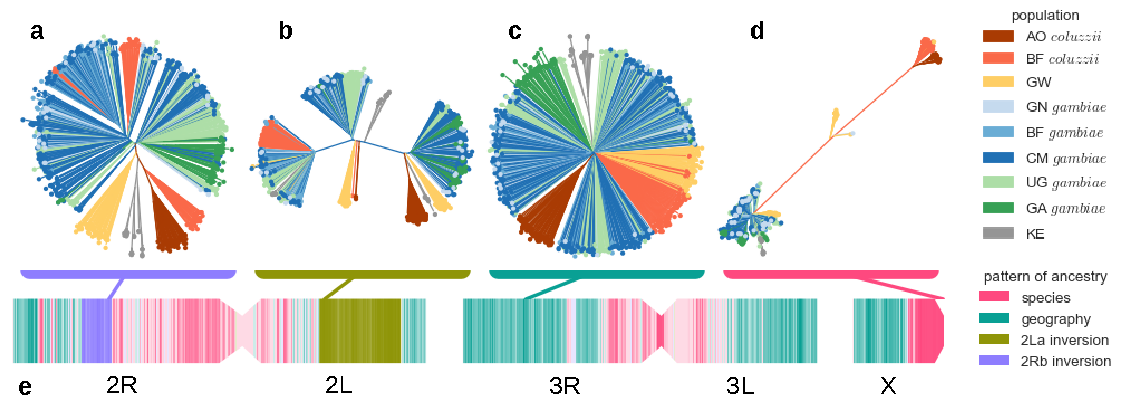
\includegraphics[width=1.1\textwidth,center]{artwork/chapter4/treescan.pdf}
\caption{Variation across the genome in patterns of relatedness between individual mosquitoes.
%
Panels \textbf{a-d} each show a neighbour-joining tree computed from pairwise genetic distances within a specific 200 kb genomic window, illustrating the four most common patterns of relatedness found throughout the genome.
%
Each node in the tree represents a single individual, coloured by population.
%
\textbf{a}, Example of tree within the 2Rb inversion.
%
\textbf{b}, Example of tree within the 2La inversion.
%
\textbf{a}, Example of tree from euchromatic region of Chromosome 3.
%
\textbf{a}, Example of tree pericentromeric region of the X chromosome.
%
\textbf{e}, Painting of the genome illustrating where the four major patterns of relatedness are found.
%
Each 200 kb window is painted with a colour to indicate which of the four major patterns of relatedness it is most strongly correlated with.
%
}
\label{fig:treescan}
\end{figure}


To explore the relationship between genetic population structure and genome architecture, I divided the genome into non-overlapping 200 kb windows, and then computed pairwise genetic distance between individuals within each window separately.
%
For each window I computed a neighbour-joining tree and visualised each of the resulting trees as an unrooted dendrogram.
%
Several qualitatively different tree topologies were evident in different genome regions (e.g., Fig.~\ref{fig:treescan}a-d).
%
For example, within the pericentromeric region of the X chromosome, trees showed extremely strong clustering by species (e.g., Fig.~\ref{fig:treescan}d).
%
In contrast, trees from euchromatic regions of Chromosome 3 showed some clustering by geographical location, but no clustering by species at all (e.g., Fig.~\ref{fig:treescan}c).
%
Trees within the 2Rb and 2La inversions also had unique topologies, consistent with clustering by inversion karyotype (e.g., Fig.~\ref{fig:treescan}a,b).


To analyse these variations in tree topology systematically, I computed the Pearson correlation coefficient between genetic distance matrices from all pairs of genomic windows.
%
I then performed dimensionality reduction on the resulting correlation matrix via multidimensional scaling, to identify common patterns of relatedness found in multiple genome windows.
%
The first three principal coordinates (PCs) from this analysis displayed a strong association with specific patterns of relatedness and genome regions.
%
To visualise these results, I devised a transformation from these first three PCs to different colours representing the different patterns of relatedness, and used these to paint the associated genome windows (Fig.~\ref{fig:treescan}e).
%
The first PC identified the common pattern of relatedness found throughout the 2La inversion.
%
The third PC identified the pattern of relatedness found within the 2Rb inversion.
%
The second PC identified the contrast between the highly species-driven patterns of relatedness found generally in pericentromeric regions, particularly of the X chromosome, and the more geographically-driven patterns found in euchromatic regions of X chromosome and Chromosome 3.
%
There were also a minority of genome windows which did not display a strong correlation any of the four major patterns of relatedness, shown in Fig~\ref{fig:treescan}e as paler colours.
%
These included the windows spanning the insecticide resistance gene \textit{Vgsc} which is found near to the centromere of chromosome arm 2L, and which is known to have experienced adaptive introgression between \textit{An. gambiae} and \textit{An. coluzzii}~\parencite{Clarkson2014,Norris2015}.
%
This provides a clue that windows affected by strong positive selection may display unusual patterns of relatedness due to adaptive gene flow between countries and/or species, explored further in Chapter 6.


It is still not clear why we observe such a stark contrast between the pericentromeric and euchromatic regions of the X chromosome, and to a lesser extent Chromosome 3.
%
One factor that undoubtedly plays some part is the reduction in the rate of recombination towards the centromeres~\parencite{Cruickshank2014}.
%
Reduced recombination means that selection at linked sites will play a stronger role.
%
This includes purifying selection, which acts to reduce genetic diversity and could accelerate the fixation of different alleles between the two species.
%
In the previous chapter we saw clearly that the level of nucleotide variation was much reduced towards pericentromeric genome regions.
%
This could also include positive selection for speciation genes.
%
The genes involved in maintaining differentiation between \textit{An. gambiae} and \textit{An. coluzzii} still remain a mystery, but if one or more key genes were located towards the pericentromeric region of the X chromosome, then they would be expected to have a substantial effect on the surrounding genome region.
%
\textit{An. gambiae} and \textit{An. coluzzii} hybrids are fully fertile, and the two species are known to undergo some hybridisation in natural populations, the degree of which may vary over both space and time~\parencite{Weetman2012,Lee2013}.
%
However, genome regions linked to speciation genes would display very little if any evidence for gene flow between the species due to selection against hybrids, whereas unlinked regions would be much less constrained and alleles could move more freely.
%
In any case, resolving the causes of these contrasting patterns of relatedness is beyond the scope of this thesis, and remains an area of active research and debate.
%
For the present purposes, I continued my investigation of population structure, diversity and differentiation using only the euchromatic regions of Chromosome 3, because this is unaffected by large polymorphic inversions or regions of reduced recombination.


%%%%%%%%%%%%%%%%%%%%%%%%%%%%%%%%%%%%%%%%%%%%%%%%%%%%%%%%%%%%%%%%%%%%%%%%%%%%%%%
%%%%%%%%%%%%%%%%%%%%%%%%%%%%%%%%%%%%%%%%%%%%%%%%%%%%%%%%%%%%%%%%%%%%%%%%%%%%%%%
\subsection{Population structure}\label{subsec:pop-structure}


To further explore patterns of genetic population structure I used SNPs from euchromatic regions of Chromosome 3 to perform a principal components analysis (PCA)~\parencite{Patterson2006} (Fig.~\ref{fig:pca}).
%
This analysis is a form of dimensionality reduction, and condenses the information present in the hundreds of thousands of SNPs into a smaller number of principal components (PCs) that explain the maximum amount of variance within the data.
%
When applied to genetic variation data, each principal component usually identifies two or more groupings of individuals, such that genetic relatedness is higher within groups than between them.
%
PCA in fact has a direct genealogical interpretation, and under certain conditions each principal component will capture a historical divergence between populations~\parencite{McVean2009}.
%
In practice the interpretation of PCA is not always so simple, because demographic complexities such as admixture events and technical factors such as variations sample size will affect the shape of the result.
%
Nevertheless, PCA allows us to identify genetically distinct populations, by examining how samples group together within the highest PCs.


\begin{figure}[t!]
\centering
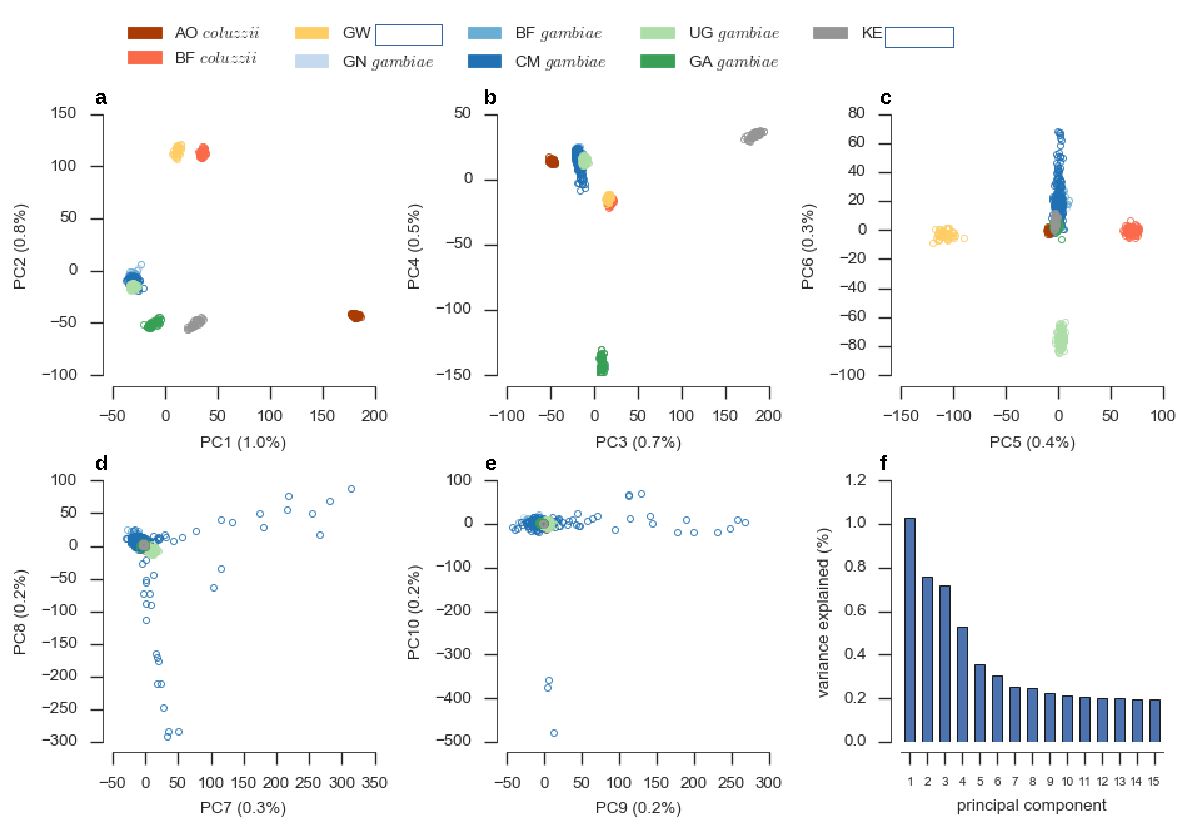
\includegraphics[width=1.1\textwidth,center]{artwork/chapter4/pca.pdf}
\caption{Principal components analysis of SNP genotypes in the 765 wild-caught mosquitoes in the Ag1000G phase 1 cohort.
%
\textbf{a--e}, Scatter plots show principal components (PCs) 1--10, each marker is an individual mosquito.
%
\textbf{f}, Bar plot shows the variance explained by the first 15 PCs.
%
}
\label{fig:pca}
\end{figure}


The first four PCs were clearly elevated above lower PCs in the amount of variance explained, and between them revealed six distinct groupings of individuals~(Fig.~\ref{fig:pca}).
%
These six groups revealed both geographical and species divisions.
%
Within \textit{An. gambiae}, individuals from Gabon formed a distinct group, and the remaining individuals from Guinea, Burkina Faso, Cameroon and Uganda grouped together.
%
Within \textit{An. coluzzii}, individuals from Burkina Faso and Angola each formed a distinct group.
%
The two remaining groups comprised individuals from Guinea-Bissau and Kenya respectively.
%
The species status of these two groups was uncertain, because individuals from Guinea-Bissau displayed a mixture of species genotypes according to conventional molecular assays, and those assays were not performed on the Kenyan samples.
%
I return to the question of species assignment for these groups below.
%
PC5 revealed a further split within \textit{An. gambiae} between Uganda and the remaining individuals.
%
PC6 emphasized the distinction between Burkina Faso \textit{An. coluzzii} and Guinea-Bissau, which were visibly distinct also in higher components but to a lesser degree.
%
PCs 7--10 all displayed some structuring among the Cameroon \textit{An. gambiae}, with individuals from the southern-most collection site spreading out away from the main group of individuals collected from the other more northerly sites.


%%%%%%%%%%%%%%%%%%%%%%%%%%%%%%%%%%%%%%%%%%%%%%%%%%%%%%%%%%%%%%%%%%%%%%%%%%%%%%%
%%%%%%%%%%%%%%%%%%%%%%%%%%%%%%%%%%%%%%%%%%%%%%%%%%%%%%%%%%%%%%%%%%%%%%%%%%%%%%%
\subsection{Population differentiation}\label{subsec:pop-diff}


To further investigate genetic population structure, I computed the pairwise average $F_{ST}$ between all pairs of populations defined by species and country (Fig.~\ref{fig:popdiff}a).
%
The $F_{ST}$ statistic summarises the extent to which allele frequencies differ between two groups of individuals, and provides information about the degree of differentiation between the two sampled populations~\parencite{Rousset1997,Holsinger2009,Bhatia2013}.
%
In general, higher $F_{ST}$ values indicate a lower rate of gene flow and greater genetic drift between two populations.
%
I also computed the rate of doubleton ($f_{2}$) variant sharing between the same pairs of populations (Fig.~\ref{fig:popdiff}b).
%
Doubleton variants are those where the alternate allele is only observed twice.
%
In general, doubleton variants are likely to be enriched for recent mutations, because it takes longer time for alleles to reach higher frequencies.
%
Thus patterns of sharing of doubleton variants between individuals are more indicative of recent patterns of relatedness~\parencite{1000G2012}.


\begin{figure}[t!]
\centering
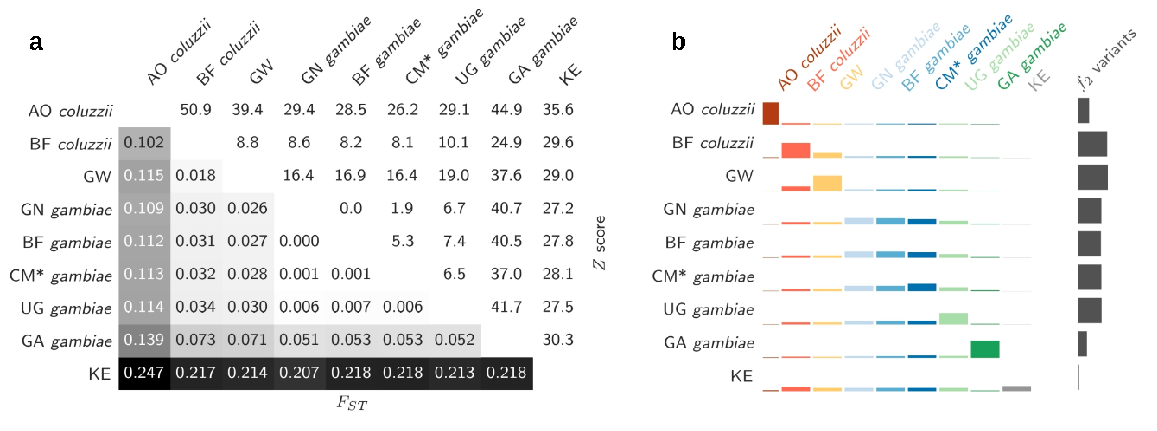
\includegraphics[width=1.1\textwidth,center]{artwork/chapter4/popdiff.pdf}
\caption{Measures of genetic differentiation between pairs of populations defined by species and country of collection, using SNPs from euchromatic regions of Chromosome 3.
%
\textbf{a}, Pairwise average $F_{ST}$.
%
The lower triangle shows $F_{ST}$ values, the upper triangle shows $Z$ scores computed using the block-jackknife process described by \textcite{Bhatia2013}.
%
\textbf{b}, Doubleton ($f_2$) variant sharing between populations.
%
Each bar shows the number of doubleton variants shared between two populations (or found within a single population on the diagonal).
%
Bar heights are normalised within each row to show the relative rate of doubleton sharing with other populations.
%
Grey bars at the right margin show the total numbers of doubleton variants found for each population.
%
}
\label{fig:popdiff}
\end{figure}


These analyses confirmed relatively strong differentiation between Gabon and other \textit{An. gambiae} populations, with $F_{ST} > 0.051$.
%
In contrast, $F_{ST}$ values between the other four \textit{An. gambiae} populations were an order of magnitude smaller, at most 0.007.
%
The degree of differentiation between Gabon and other \textit{An. gambiae} populations was greater than that found between the two species within Burkina Faso, where both species were sampled at the same location ($F_{ST} = 0.031$).
%
The higher $F_{ST}$ values involving Gabon cannot simply be a reflection of greater geographical distance, because the distance between Uganda and \textit{An. gambiae} populations to the west is greater, yet $F_{ST}$ values are much lower.
%
These results indicate that the Gabon individuals are separated by other \textit{An. gambiae} populations to the north by some significant barrier to gene flow.
%
The obvious candidate for such a barrier is the equatorial rainforest, which represents a major ecological discontinuity.
%
Similarly, \textit{An. coluzzii} from Angola were highly differentiated from \textit{An. coluzzii} from Burkina Faso ($F_{ST} = 0.102$).
%
Again, the level of differentiation was greater than that between the two species within Burkina Faso.
%
Angola is the southern-most sampling location in the Ag1000G phase 1 cohort, and provides further support for a north/south ecogeographical barrier between mosquito populations, affecting both species.


A surprising result was the near-total lack of differentiation between the \textit{An. gambiae} populations from Guinea, Burkina Faso and Cameroon, with $F_{ST}$ reaching at most 0.001 and barely achieving statistical significance (Fig.~\ref{fig:popdiff}a).
%
This result was also supported by the doubleton analysis, with near-equal rates of doubleton sharing both within and between these populations (Fig.~\ref{fig:popdiff}b).
%
The lack of differentiation indicates high rates of gene flow, but this is surprising because the physical distances are considerable, with 2,170 km separating sampling sites in Cameroon and Burkina Faso, and 640 km separating sampling sites in Burkina Faso from Guinea.
%
Previously, accepted wisdom was that anopheline mosquitoes disperse at most 5 km during their lifetime~\parencite{Service1997}, and therefore we would expect to see some geographical isolation by distance between these locations~\parencite{Rousset1997}.
%
This is being challenged by recent observations of anopheline mosquitoes including \textit{An. coluzzii} engaging in what appears to be purposeful wind-assisted long-distance migration~\parencite{Huestis2019}.
%
However, the evidence is conflicting, as studies in the same geographical region indicate that \textit{An. gambiae} is more likely to engage in migratory behaviour, whereas \textit{An. coluzzii} appears to cope with highly seasonal availability of breeding habitat by aestivation~\parencite{Dao2014}.
%
Unfortunately, Ag1000G phase 1 includes only limited geographical sampling of \textit{An. coluzzii}, and so it is not possible to make a comparison between the two species at this stage.
%
Subsequent project phases will expand sampling of both species and provide richer opportunities to investigate gene flow questions.


The Kenyan population displayed a high level of differentiation ($F_{ST} > 0.207$) with all other populations, with similar $F_{ST}$ values against populations of both species.
%
The Kenyan samples were expected to be genetically isolated to a certain degree, being sampled on the coast at the most easterly location among the collection sites, and being the only samples collected to the east of the Rift Valley, which presents a natural geographical barrier to gene flow.
%
However, the magnitude of this difference was surprising, being more than twice that found between most other population pairs.
%
This could indicate extremely low rates of gene flow, but could also be an effect of strong genetic drift within the Kenyan population, which would be consistent with analyses of genetic diversity presented below.
%
The fact that the Kenyan population was equally differentiated from both \textit{An. gambiae} and \textit{An. coluzzii} was also surprising, given that the Kenyan samples were believed to be \textit{An. gambiae}, explored further below in the sub-section on gene flow between species.


%%%%%%%%%%%%%%%%%%%%%%%%%%%%%%%%%%%%%%%%%%%%%%%%%%%%%%%%%%%%%%%%%%%%%%%%%%%%%%%
%%%%%%%%%%%%%%%%%%%%%%%%%%%%%%%%%%%%%%%%%%%%%%%%%%%%%%%%%%%%%%%%%%%%%%%%%%%%%%%
\subsection{Genetic diversity within populations}\label{subsec:diversity}


In the previous chapter I performed an initial analysis of genetic diversity, computing nucleotide diversity ($\pi$) within the Ag1000G phase 1 cohort as a whole.
%
This analysis of course ignored the fact that different populations within a species may exhibit different levels of genetic diversity, due to differences in their demographic history such as contractions or expansions in population size.
%
To investigate population differences in genetic diversity I performed four further analyses within each of nine populations defined by country and species (Fig.~\ref{fig:diversity}).
%
The first of these analyses computed $\pi$, which summarises the fraction of nucleotide differences between pairs of chromosomes within a population (Fig.~\ref{fig:diversity}a).
%
The second analyses computed Tajima's $D$, which summarises the distribution of allele frequencies within a population (Fig.~\ref{fig:diversity}b).
%
The third analysis computed the full site frequency spectrum (SFS) for each population, which provides information about how many SNPs are observed at different allele frequencies (Fig.~\ref{fig:diversity}c).
%
The final analysis examined the decay of linkage disequilibrium, which summarised the degree to which genotypes are correlated at pairs of SNPs at different physical distances from each other (Fig.~\ref{fig:diversity}d).


\begin{figure}[t!]
\centering
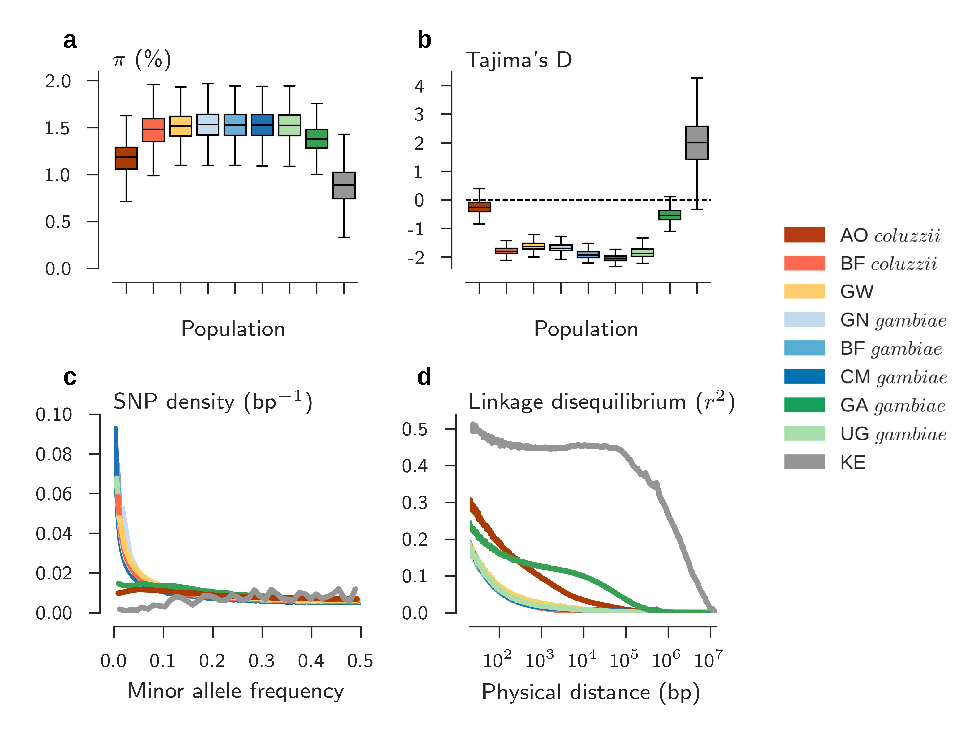
\includegraphics[width=0.9\textwidth]{artwork/chapter4/pop_params.pdf}
\caption{Genetic diversity within populations, computed using SNP genotypes from Chromosome 3.
%
\textbf{a}, Nucleotide diversity, computed for each population in 20 kb windows.
%
\textbf{b}, Tajima's $D$, computed in 20 kb windows.
%
\textbf{c}, Folded site frequency spectra, normalised such that a population with stable population size is expected to show equal SNP density across all minor allele frequencies.
%
\textbf{d}, Decay of linkage disequilibrium, averaged over pairs of randomly sampled SNPs at different physical distances.
%
}
\label{fig:diversity}
\end{figure}


These analyses revealed strong contrasts between populations in both the magnitude and architecture of genetic diversity.
%
All the populations to the north of the equatorial rainforest, from Guinea-Bissau in the West to Uganda in the East, including both species, displayed very similar results, with the highest genome-wide average $\pi = 1.5\%$, Tajima's $D < -1.5$, SFS with a strong excess of SNPs at low minor allele frequency, and LD decaying to background levels within 2 kb.
%
These characteristics indicate large effective population size and are also consistent with a major population expansion at some point within their history.
%
In both Gabon \textit{An. gambiae} and Angola \textit{An. coluzzii}, $\pi$ was lower, Tajima's $D$ was approaching zero, SFS were more balanced and LD decay was $> 10$ kb.
%
These characteristics are consistent with an effective population size that is both smaller and has been more stable over time.
%
The Kenyan population displayed the most extreme patterns of diversity, with the lowest $\pi$, Tajima's $D > 2$, SFS with a deficit of SNPs at lower minor allele frequencies, and LD not decaying to background until $> 10$ Mb.
%
These characteristics indicate a strong and recent reduction in effective population size.
%
Further examination of levels of heterozygosity within individuals revealed that Kenyan mosquitoes displayed long runs of homozygosity, in some cases affecting almost entire chromosome arms, a pattern not observed in mosquitoes from any other population (Fig.~\ref{fig:keroh}).
%
Such patterns of homozygosity are usually only observed after multiple generations of inbreeding, similar to patterns found in domesticated animals (e.g.~\cite{Purfield2012}) and mosquitoes maintained in lab colonies for several years.


%%%%%%%%%%%%%%%%%%%%%%%%%%%%%%%%%%%%%%%%%%%%%%%%%%%%%%%%%%%%%%%%%%%%%%%%%%%%%%%
%%%%%%%%%%%%%%%%%%%%%%%%%%%%%%%%%%%%%%%%%%%%%%%%%%%%%%%%%%%%%%%%%%%%%%%%%%%%%%%
\subsection{Genetic variation within Cas9 gene drive targets}\label{subsec:gene-drive}


The high level of nucleotide diversity within many of the mosquito populations sampled in Ag1000G phase 1 is interesting in its own right, but also has practical consequences for the development of new vector control tools based on gene drives.
%
Gene drives are a promising future technology for mosquito control, whereby an engineered genetic element is integrated into the mosquito genome that has the capability to be transmitted to progeny with super-Mendelian inheritance~\parencite{Burt2003}.
%
Because of this biased inheritance, a gene drive will propagate itself within a mosquito population, even if it is in some way deleterious to its carrier.
%
For example, gene drives have been engineered and proven effective under lab conditions which cause population suppression by biasing the sex ratio among offspring to be almost all male~\parencite{Kyrou2018}.
%
Current gene drives make use of CRISPR/Cas9 homing endonucleases, which can be engineered to target almost any gene, because they include a guide RNA which matches a 21 bp sequence in the target genome.
%
The guide RNA can be designed to match any sequence of 18 nucleotides, then must terminate with the protospacer adjacent motif (PAM).
%
However, any natural genetic variation in the target sequence within the mosquito population could reduce efficacy of a gene drive, because it will affect binding of the Cas9 guide RNA.
%


\begin{figure}[t!]
\centering
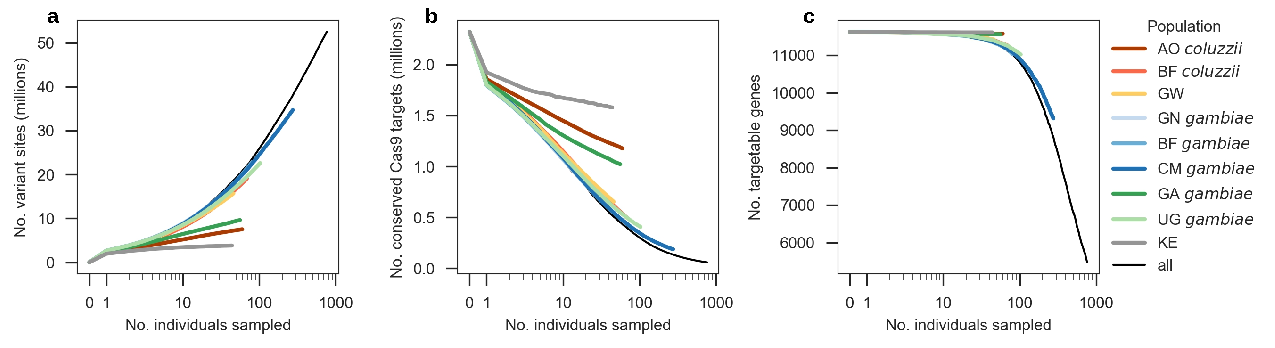
\includegraphics[width=1.1\textwidth,center]{artwork/chapter4/cas9_targets.pdf}
\caption{Genetic diversity and its impact on the availability of conserved Cas9 targets for the design of gene drives.
%
\textbf{a}, Numbers of sites with nucleotide variation across the whole genome.
%
\textbf{b}, Numbers of Cas9 targets with no nucleotide variation.
%
\textbf{c}, Numbers of genes containing at least one conserved Cas9 target site.
%
}
\label{fig:cas9}
\end{figure}


I explored the impact of nucleotide variation on the availability of highly conserved Cas9 target sequences, in collaboration with Ag1000G Consortium members Mara Lawniczak and Krzysztof Kozak.
%
I was particularly interested to explore the impact of sample size and of population differences in levels of genetic diversity on the ascertainment of viable Cas9 gene drive target sites.
%
I performed an analysis whereby I identified all 21 bp sequences in the reference genome terminating in a PAM motif, within which no nucleotide variation was found within a given Ag1000G phase 1 population.
%
I repeated this multiple times with successively greater down-sampling of individuals from each population.
%
I then plotted for each population the number of variant sites (Fig.~\ref{fig:cas9}a), the number of conserved Cas9 targets (Fig.~\ref{fig:cas9}b) and the number of genes containing at least one viable Cas9 target (Fig.~\ref{fig:cas9}c), and how these metrics varied with increasing sample size.
%
These analyses showed that the higher levels of nucleotide diversity among the populations sampled to the north of the equatorial rainforest had a dramatically greater impact on the reduction of available Cas9 targets, compared with the more southerly populations from Gabon and Angola, and the Kenyan population.
%
At a sample size of 50, more than 1.5 million Cas9 targets remained conserved in Kenya, and more than 1 million were conserved in Angola and Gabon, whereas less than 0.5 million were conserved in any of the remaining populations.
%
Within the whole cohort, less than 3\% of Cas9 targets were fully conserved at the nucleotide level.
%
Clearly some \textit{An. gambiae} and \textit{An. coluzzii} populations will be more naturally resistant to gene drives than others due to higher diversity, and will require more intensive sampling in order to survey existing variation and design gene drives to accommodate this.


%%%%%%%%%%%%%%%%%%%%%%%%%%%%%%%%%%%%%%%%%%%%%%%%%%%%%%%%%%%%%%%%%%%%%%%%%%%%%%%
%%%%%%%%%%%%%%%%%%%%%%%%%%%%%%%%%%%%%%%%%%%%%%%%%%%%%%%%%%%%%%%%%%%%%%%%%%%%%%%
\subsection{Gene flow between species}\label{subsec:species}


% https://github.com/malariagen/ag1000g/blob/master/notebooks/aliman/20150526%20Admixture%2C%20f3%2C%20D.ipynb

% https://github.com/malariagen/ag1000g/blob/master/notebooks/aliman/20150529%20Admixture%2C%20introgression.ipynb

% https://github.com/malariagen/ag1000g/blob/master/notebooks/aliman/20150726%20Kenya%20ancestral%20or%20admixed%3F.ipynb


A long-standing question in the field is the extent to which gene flow occurs via hybridisation between species within the \textit{An. gambiae} complex.
%
I investigated genome-wide evidence for gene flow between species using data from Ag1000G phase 1, combined with data from \textit{An. arabiensis} and outgroup species from \textcite{Neafsey2015}.
%
I used the $f_3$ and $f_4$ statistics which test for evidence of admixture, as defined by \textcite{Patterson2012}.
%
The $f_3$ statistic tests if allele frequencies in a population with suspected admixture are on average intermediate between two donor populations.
%
The $f_4$ statistic, also known as the ABBA-BABA test or Patterson's $D$, tests for unbalanced allele sharing in a four population tree.
%
In this subsection to be concise when describing different $f_4$ tests I use population abbreviations of the form \{country code\}-\{species\}, e.g., ``BF-gam'' is Burkina Faso \textit{An. gambiae}, ``AO-col'' is Angola \textit{An. coluzzii}, ``GW'' is Guinea-Bissau, etc., and ``O'' denotes the outgroup species \textit{An. christyi}.


Hybrids between \textit{An. gambiae} and \textit{An. coluzzii} are fully fertile and several studies have found evidence that hybridisation occurs at a rate that varies over both time and space~\parencite{Lee2013,Weetman2012}.
%
In Ag1000G phase 1, the samples from Guinea-Bissau displayed a mixture of species genotypes according to conventional molecular diagnostics, including individuals with an apparent hybrid genotype.
%
Similar results have been obtained from previous studies in the Far West region, and have been interpreted as evidence for a localised breakdown in reproductive isolation between \textit{An. gambiae} and \textit{An. coluzzii}~\parencite{Oliveira2008,Marsden2011,Weetman2012,Gordicho2014,Vicente2017}.
%
Ag1000G Consortium member Giordano Botta investigated this further using data from Ag1000G phase 1, showing that Guinea-Bissau individuals had a mixture of species genotypes across ancestry-informative markers on all chromosome arms~\parencite{Ag1000G2017}.
%
There are several possible explanations for these data, however, including contemporary or historical admixture between species, and retention of ancestral variation.
%
The results from PCA suggest that the Guinea-Bissau individuals are not the result of ongoing hybridisation between species, because all individuals form a single group distinct from groups of each species from nearby countries (Fig.~\ref{fig:pca}), rather than being spread out between them as would be expected under recent admixture.
%
Consistent with this, results of $f_3$ tests with Guinea-Bissau as putatively admixed and Burkina Faso \textit{An. gambiae} and \textit{An. coluzzii} as donor populations were significantly positive, indicating allele frequencies in Guinea-Bissau were not intermediate and arguing against a simple admixture scenario.
%
The Guinea-Bissau population was most closely related to the Burkina Faso \textit{An. coluzzii} population in PCA, $F_{ST}$ and doubleton sharing analyses (Figs.~\ref{fig:pca},~\ref{fig:popdiff}).
%
$f_4$ tests of the form D(GW, BF-col; GN-gam; O) were balanced and did not provide any significant evidence for admixture between Guinea-Bissau and Guinea \textit{An. gambiae} on any chromosome, except for the pericentromeric region of the X chromosome (Table~\ref{table:gwf4}; Fig.~\ref{fig:gwf4}).
%
Taken together, these results show that the origins of the Guinea-Bissau population and its relationships with \textit{An. gambiae} and \textit{An. coluzzii} populations are more complex than previously appreciated, and caution against over-interpretation of data from conventional species diagnostics.


A surprising result from the AIM analysis was that the Kenyan individuals also had a mixture of \textit{An. gambiae}, \textit{An. coluzzii} and heterozygous genotypes, similar to Guinea-Bissau~\parencite{Ag1000G2017}.
%
The range of \textit{An. coluzzii} is not known to extend to the east of the Rift Valley, and so the Kenyan population cannot be the result of any recent admixture between species.
%
$f_3$ tests with Kenya as putatively admixed and all other pairs of populations as putative donors did not support evidence for admixture.
%
I also computed $f_4$ statistics for the Kenyan population, using \textit{An. gambiae} and \textit{An. coluzzii} from Burkina Faso as potential sibling populations and \textit{An. Christyi} as the outgroup.
%
These analyses gave conflicting results depending on which chromosome arm was analysed, with 3R indicating that Kenya was sister with \textit{An. coluzzii} (\textit{D(KE, BF-col; BF-gam, O)}; $Z=0.1$), 3L indicating Kenya was a cryptic taxon ancestral to both species (D(BF-gam, BF-col; KE, O); Z=-0.7) and the X chromosome not providing clear support for any one hypothesis.
%
Thus, the origins and species status of the Kenyan population are also uncertain.
%
These results reinforce the fact that reliance on a single diagnostic marker to identify species is very limiting and may be missing important signals of introgression or cryptic taxa.


Among the remaining populations, the AIMs supported a clear assignment of \textit{An. gambiae} or \textit{An. coluzzii} species status, in agreement with conventional molecular diagnostics~\parencite{Ag1000G2017}.
%
However, this does not rule out low level gene flow between species, and among these populations there was clear evidence for a greater degree of gene flow in some populations relative to others.
%
All $f_4$ tests with \textit{An. coluzzii} from Angola and Burkina Faso as sister populations provided significant evidence for admixture between Angola and \textit{An. gambiae}, with the strongest signal obtained for Gabon (e.g., D(AO-col, BF-col; GA-gam, O); $Z=14.0$).
%
Conversely, all tests with two \textit{An. gambiae} populations as sisters provided evidence for admixture between Gabon \textit{An. gambiae} and \textit{An. coluzzii}, with the strongest signal obtained for Angola (e.g., D(GA-gam, GN-gam; AO-col, O); $Z=11.1$).
%
These results show that gene flow between the two species has been stronger in southerly populations than northerly populations, and that it has been bidirectional.


Hybridisation between \textit{An. gambiae} and \textit{An. arabiensis} is also known to occur in nature but thought to be less common~\parencite{White1971,Coluzzi1979,dellaTorre1997}.
%
I used $f_4$ tests of the form D(X, Y; A, O), where X and Y were all pairs of Ag1000G phase 1 populations, and A was \textit{An. arabiensis} from \textcite{Neafsey2015}, to investigate whether gene flow with \textit{An. arabiensis} is greater for some populations relative to others.
%
These tests were significant in some cases (e.g., D(BF-gam, BF-col; A, O); $Z=8.0$; D(UG-gam, BF-gam; A, O); $Z=6.9$) but not others, allowing for a partial ordering of populations by relative degree of introgression .
%
This partial ordering was GW < \{AO-col, BF-col\} < \{GN-gam, BF-gam, CM-gam, GA-gam\} < UG-gam < KE, indicating that introgression with \textit{An. arabiensis} is higher in \textit{An. gambiae} relative to \textit{An. coluzzii}, and higher in easterly populations relative to westerly populations.


%%%%%%%%%%%%%%%%%%%%%%%%%%%%%%%%%%%%%%%%%%%%%%%%%%%%%%%%%%%%%%%%%%%%%%%%%%%%%%%
%%%%%%%%%%%%%%%%%%%%%%%%%%%%%%%%%%%%%%%%%%%%%%%%%%%%%%%%%%%%%%%%%%%%%%%%%%%%%%%
%%%%%%%%%%%%%%%%%%%%%%%%%%%%%%%%%%%%%%%%%%%%%%%%%%%%%%%%%%%%%%%%%%%%%%%%%%%%%%%
\section{Conclusions}\label{sec:ch4-conclusions}


In this chapter I have showed that there are clear patterns of genetic structure among the populations sampled in the Ag1000G phase 1 cohort.
%
These patterns of population structure are also associated with differences in the magnitude and architecture of genetic diversity within populations.
%
Taken together, these results point to complex and varied demographic histories, and multiple biological and geographical factors affecting population size and rates of gene flow between populations and species.
%
Within both species there is a strong north/south divide, with high differentiation between populations on either side of the equatorial rainforest, higher genetic diversity and evidence for a major population expansion in northerly but not southerly populations.
%
Within \textit{An. gambiae} there appears to be an extremely high rate of gene flow between the northerly populations, despite substantial physical distance, raising important questions about the rate and range of migration within this species.
%
There are also unusual populations in both the far West and far East, where individuals carry an apparent mixture of species ancestry, but this cannot be explained by a simple model of recent admixture between species.
%
We also see an extreme contrast between populations on either side of the East African Rift, with evidence for a recent and substantial population bottleneck in the Kenyan population.
%
Clearly there are limits to the extent to which these findings can be generalised, because geographical sampling is limited particularly within \textit{An. coluzzii}, and much remains to be learned about both of these species throughout their complete geographical ranges.
%
However, these results show that there are important heterogeneities within these species, which are of basic biological interest, but also relevant to malaria vector population surveillance, because they will affect factors such as the efficacy of gene drives for population suppression, or the speed, direction and extent to which insecticide resistance mutations spread.
%
In the next chapter I investigate each of these populations in more detail, focusing on their evolutionary history and searching for genome regions evolving rapidly due to positive selection for insecticide resistance.


%%%%%%%%%%%%%%%%%%%%%%%%%%%%%%%%%%%%%%%%%%%%%%%%%%%%%%%%%%%%%%%%%%%%%%%%%%%%%%%
%%%%%%%%%%%%%%%%%%%%%%%%%%%%%%%%%%%%%%%%%%%%%%%%%%%%%%%%%%%%%%%%%%%%%%%%%%%%%%%
%%%%%%%%%%%%%%%%%%%%%%%%%%%%%%%%%%%%%%%%%%%%%%%%%%%%%%%%%%%%%%%%%%%%%%%%%%%%%%%
\section{Methods}\label{sec:ch4-methods}


In order to facilitate the population genetic analyses described in this chapter on the relatively large Ag1000G SNP variation data, I developed a new software package named scikit-allel\footnote{https://github.com/cggh/scikit-allel} for the Python programming language.
%
scikit-allel aims to support a range of standard data manipulations and statistical functions that are useful for exploratory analysis of large-scale genome variation data, with implementations that are sufficiently performant and scalable such that those analyses can be run interactively, allowing rapid iteration and hypothesis generation.
%
To achieve this, scikit-allel builds on several high-performance general-purpose scientific computing libraries, including NumPy~\parencite{Harris2020}, SciPy~\parencite{Virtanen2020}, Cython~\parencite{Behnel2011}, Pandas~\parencite{McKinney2010} and Matplotlib~\parencite{Hunter2007}.
%
The sub-sections below provide further details of specific analyses.
%
Unless otherwise stated, analyses were performed using scikit-allel and custom Python notebooks.


%%%%%%%%%%%%%%%%%%%%%%%%%%%%%%%%%%%%%%%%%%%%%%%%%%%%%%%%%%%%%%%%%%%%%%%%%%%%%%%
%%%%%%%%%%%%%%%%%%%%%%%%%%%%%%%%%%%%%%%%%%%%%%%%%%%%%%%%%%%%%%%%%%%%%%%%%%%%%%%
\subsection{Genetic distance analyses}\label{subsec:methods-genetic-distance}

To investigate variations in patterns of relatedness between individuals across the genome, I divided the genome into 1,418 contiguous non-overlapping windows, where each window contained 100 kb of accessible positions (equally-accessible windows).
%
Within each window I computed the city-block distance between all pairs of individuals, producing a $765 \times 765$ distance matrix.
%
I used these distance matrices to compute and plot a neighbour-joining tree for each window via the ape package version 3.5 for R~\parencite{Popescu2012}.
%
To compare these distance matrices systematically, I computed the Pearson correlation coefficient between all pairs of distance matrices, producing a $1418 \times 1418$ correlation matrix.
%
I converted this to a distance matrix by computing $\sqrt{(1-r^{2})}$ where $r$ is the correlation coefficient, and performed a singular value decomposition (SVD) on this matrix.
%
I then plotted the first ten components from this transformation against position in the genome.
%
To provide a visual representation of this transformation in Fig.~\ref{fig:treescan}b I painted the genome as follows.
%
Within the 2La inversion I painted with one colour, using the value from the first SVD component
rescaled between 0 and 1 as the alpha value.
%
Within the 2Rb inversion I painted with a second colour, using the value from the third SVD component rescaled between 0 and 1 as the alpha value.
%
Within the remainder of the genome I painted with either a third or a fourth colour, depending on whether the value of the second SVD component was positive or negative.
%
Positive and negative values were separately rescaled between 0 and 1 to provide alpha values.


%%%%%%%%%%%%%%%%%%%%%%%%%%%%%%%%%%%%%%%%%%%%%%%%%%%%%%%%%%%%%%%%%%%%%%%%%%%%%%%
%%%%%%%%%%%%%%%%%%%%%%%%%%%%%%%%%%%%%%%%%%%%%%%%%%%%%%%%%%%%%%%%%%%%%%%%%%%%%%%
\subsection{Principal components analysis}\label{subsec:methods-pca}


SNPs for inclusion in principal components analysis were chosen by selecting biallelic variants from within the regions 3R:1-37 Mbp and 3L:15-41 Mbp.
%
Only variants with minor allele frequency $>=1\%$ were retained and each chromosome arm was randomly down-sampled to 100,000 variants.
%
I then pruned to remove SNPs in linkage disequilibrium, excluding SNPs above an $r^2$ threshold of 0.01 in moving windows of 500 SNPs with a step size of 250 SNPs.
%
SNPs from both chromosome arms were then concatenated, and PCA was run following methods described in \textcite{Patterson2006}.


%%%%%%%%%%%%%%%%%%%%%%%%%%%%%%%%%%%%%%%%%%%%%%%%%%%%%%%%%%%%%%%%%%%%%%%%%%%%%%%
%%%%%%%%%%%%%%%%%%%%%%%%%%%%%%%%%%%%%%%%%%%%%%%%%%%%%%%%%%%%%%%%%%%%%%%%%%%%%%%
\subsection{Population differentiation analyses}\label{subsec:methods-popdiff}


Average $F_{ST}$ was computed between all pairs of 9 populations defined by country of origin and species, except for Guinea-Bissau and Kenya which were each treated as a single population with uncertain species status.
%
Hudson's $F_{ST}$ estimator was used, and the ratio of averages computed following \textcite{Bhatia2013}.
%
Only SNPs within the regions 3R:1-37 Mbp and 3L:15-41 Mbp and which were segregating in both populations were used.
%
Standard error for each average was computed using a block-jackknife with block size 10,000 SNPs.


The 765 individuals from natural populations were grouped into 9 populations as described above for $F_{ST}$ analysis.
%
Each population was then randomly down-sampled to the size of the smallest population (Guinea \textit{An. gambiae}, N=31).
%
After down-sampling, I ascertained SNPs from Chromosome 3 with an alternate allele count of 2 (doubletons).
%
For each population, I identified the set of doubletons with at least one allele originating from an individual in that population.
%
I then computed the fraction of those doubletons shared with each other population including itself.


%%%%%%%%%%%%%%%%%%%%%%%%%%%%%%%%%%%%%%%%%%%%%%%%%%%%%%%%%%%%%%%%%%%%%%%%%%%%%%%
%%%%%%%%%%%%%%%%%%%%%%%%%%%%%%%%%%%%%%%%%%%%%%%%%%%%%%%%%%%%%%%%%%%%%%%%%%%%%%%
\subsection{Genetic diversity analyses}\label{subsec:methods-diversity}


To compute a genome-wide average value for nucleotide diversity ($\pi$) I divided the genome into non-overlapping contiguous windows where each window contained 20 kb accessible positions.
%
For each SNP (including multiallelic SNPs) I used allele counts to compute the mean number of allelic differences between all pairs of individuals within each population.
%
A value of $\pi$ was computed for each window for each population by summing the mean pair-wise differences over all SNPs in the window and dividing by the number of accessible positions.


From SNP validation experiments I estimated an FDR of 0.4\% and a sensitivity of 94.6\% (Chapter 3).
%
To explore the impact of error rates on estimates of diversity, I computed conservative lower bounds
on $\pi$ and Watterson's $\theta$ for each population under an assumption of 1\% FDR and 100\% sensitivity by randomly sampling 99\% of SNPs in the dataset without replacement.
%
I computed conservative upper bounds under an assumption of 0\% FDR and 94\% sensitivity by randomly sampling 106\% of SNPs from the dataset with replacement.
%
Values for chromosome arm 3R excluding pericentromeric regions are given in Table~\ref{table:pirange}.
%
I report unadjusted values in the results section above.


For each population, a site frequency spectrum (SFS) was computed using allele counts in SNPs from Chromosome 3 excluding pericentromeric regions.
%
Folded SFS were multiplied by the scaling factor $k (n - k) / n$ where $k$ is the minor allele count and $n$ is the number of chromosomes, to facilitate
comparison with theoretical SFS for a population with constant size (expected to have constant scaled frequency for all values of $k$).


SNPs from Chromosome 3 excluding pericentromeric regions were used for LD decay analyses.
%
For each population, the genotype correlation coefficient $r^2$~\parencite{Rogers2009} was computed for randomly sampled pairs of SNPs at a range of physical distances.
%
Only biallelic SNPs with a minor allele frequency greater than 10\% within the population were used.
%
Values were corrected for sample size by subtracting $1/n$ where $n$ is the number of sampled chromosomes.


%%%%%%%%%%%%%%%%%%%%%%%%%%%%%%%%%%%%%%%%%%%%%%%%%%%%%%%%%%%%%%%%%%%%%%%%%%%%%%%
%%%%%%%%%%%%%%%%%%%%%%%%%%%%%%%%%%%%%%%%%%%%%%%%%%%%%%%%%%%%%%%%%%%%%%%%%%%%%%%
\subsection{Admixture tests}\label{subsec:methods-admixture}


The $f_3$ and $f_4$ tests were performed using a block size of 100,000 SNPs to estimate standard error via a block jackknife procedure~\parencite{Patterson2012}.
%
$Z$ scores reported in the results are computed by dividing the test statistic by the estimated standard error, and thus indicate the number of standard deviations from zero.


%%%%%%%%%%%%%%%%%%%%%%%%%%%%%%%%%%%%%%%%%%%%%%%%%%%%%%%%%%%%%%%%%%%%%%%%%%%%%%%
%%%%%%%%%%%%%%%%%%%%%%%%%%%%%%%%%%%%%%%%%%%%%%%%%%%%%%%%%%%%%%%%%%%%%%%%%%%%%%%
%%%%%%%%%%%%%%%%%%%%%%%%%%%%%%%%%%%%%%%%%%%%%%%%%%%%%%%%%%%%%%%%%%%%%%%%%%%%%%%
\section{Acknowledgments}\label{sec:ch4-acknowledgments}


I would like to thank Nick Harding, Giordano Botta, Chris Clarkson, Tiago Antao, Krzsyztof Kozak, Daniel Schrider, Andrew Kern, Seth Redmond, Igor Sharakhov, Michael Fontaine, Martin Donnelly and Mara Lawniczak for many enlightening conversations while collaborating on population genetic analyses of the Ag1000G phase 1 data.


\clearpage
%%%%%%%%%%%%%%%%%%%%%%%%%%%%%%%%%%%%%%%%%%%%%%%%%%%%%%%%%%%%%%%%%%%%%%%%%%%%%%%
%%%%%%%%%%%%%%%%%%%%%%%%%%%%%%%%%%%%%%%%%%%%%%%%%%%%%%%%%%%%%%%%%%%%%%%%%%%%%%%
%%%%%%%%%%%%%%%%%%%%%%%%%%%%%%%%%%%%%%%%%%%%%%%%%%%%%%%%%%%%%%%%%%%%%%%%%%%%%%%
\section{Supplemental figures}\label{sec:ch4-supplemental-figures}


\begin{figure}[h!]
\centering
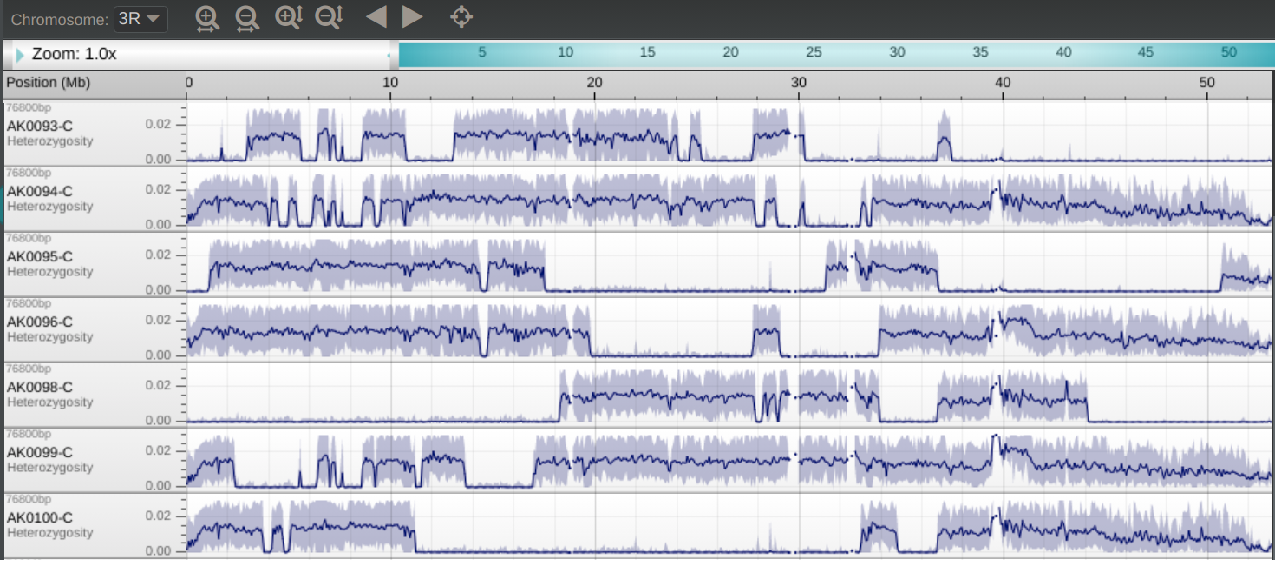
\includegraphics[width=1.1\textwidth,center]{artwork/chapter4/keroh.pdf}
\caption{Screenshot from the Panoptes Web application showing runs of homozygosity on chromosome arm 3R in a selection of seven individuals from Kenya.
%
}
\label{fig:keroh}
\end{figure}


\clearpage
\begin{figure}[h!]
\centering
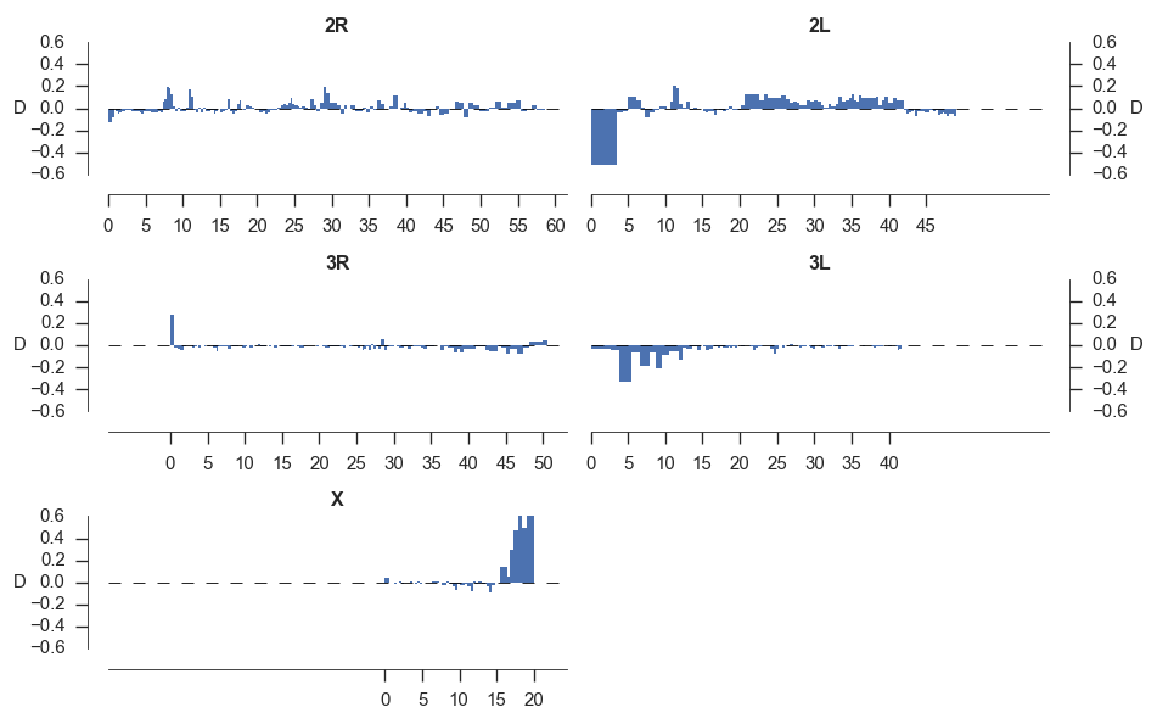
\includegraphics[width=1.1\textwidth,center]{artwork/chapter4/gwf4.pdf}
\caption{Results of the $f_4$ test D(GW, BF-col; GN-gam, O) for admixture between Guinea-Bissau (GW) and Guinea \textit{An. gambiae} (GN-gam).
%
Values for each block of 100,000 SNPs are plotted over the genome, to assess whether any particular genome regions provide evidence for admixture.
%
The only region providing strong support for admixture is the pericentromeric region of the X chromosome.
%
}
\label{fig:gwf4}
\end{figure}


\clearpage
%%%%%%%%%%%%%%%%%%%%%%%%%%%%%%%%%%%%%%%%%%%%%%%%%%%%%%%%%%%%%%%%%%%%%%%%%%%%%%%
%%%%%%%%%%%%%%%%%%%%%%%%%%%%%%%%%%%%%%%%%%%%%%%%%%%%%%%%%%%%%%%%%%%%%%%%%%%%%%%
%%%%%%%%%%%%%%%%%%%%%%%%%%%%%%%%%%%%%%%%%%%%%%%%%%%%%%%%%%%%%%%%%%%%%%%%%%%%%%%
\section{Supplemental tables}\label{sec:ch4-supplemental-tables}


\begin{table}[h]
\begin{center}
\begin{threeparttable}

\caption{Genome-wide average values for $\pi$ and $\theta_{W}$ with upper and lower bounds computed as described in Methods.
}

\label{table:pirange}

\begin{tabular}{lll}
 \hline
 \textbf{Population} & $\pi$ $(\%)$ & $\theta_{W}$  $(\%)$ \\
 \hline
AO coluzzii & 1.16 (1.14-1.23) & 1.24 (1.23-1.32) \\
BF coluzzii & 1.45 (1.44-1.54) & 3.11 (3.08-3.31) \\
GW & 1.49 (1.48-1.59) & 2.80 (2.78-2.98) \\
GN gambiae & 1.50 (1.49-1.60) & 2.82 (2.79-3.00) \\
BF gambiae & 1.50 (1.48-1.59) & 3.58 (3.54-3.80) \\
CM gambiae & 1.50 (1.49-1.59) & 4.60 (4.56-4.90) \\
GA gambiae & 1.35 (1.34-1.44) & 1.61 (1.60-1.71) \\
UG gambiae & 1.50 (1.48-1.59) & 3.51 (3.48-3.74) \\
KE & 0.87 (0.86-0.93) & 0.55 (0.55-0.59) \\
 \hline
\end{tabular}

\end{threeparttable}
\end{center}
\end{table}


\clearpage

\begin{table}[h]
\begin{center}
\begin{threeparttable}

\caption{Results of the $f_4$ test D(GW, BF-col; GN-gam, O) for admixture between Guinea-Bissau (GW) and Guinea \textit{An. gambiae} (GN-gam).
}

\label{table:gwf4}

\begin{tabular}{llrrr}
 \hline
 \textbf{Chromosome} & $D$ & $SE$ & $Z$ \\
 \hline
2R & 0.007 & 0.0048 & 1.4 \\
2L & 0.021 & 0.0093 & 2.3 \\
3R & -0.011 & 0.0039 & -2.7 \\
3L & -0.029 & 0.0067 & -4.4 \\
X & 0.078 & 0.0361 & 2.2 \\
 \hline
\end{tabular}

\end{threeparttable}
\end{center}
\end{table}


\printbibliography[
heading=subbibintoc,
title={References}
]


\end{refsection}
